\documentclass[10pt,letterpaper]{article}
\usepackage[margin=1in]{geometry}
\usepackage[latin1]{inputenc}
\usepackage{amsmath}
\usepackage{amsfonts}
\usepackage{amssymb}
\usepackage{graphicx}
\usepackage{hyperref}
\usepackage[nolist,nohyperlinks]{acronym}
\usepackage{float}
\usepackage{subcaption}

\newcommand{\SiIV}{Si\,\textsc{iv} 1403 \AA\ }
\newcommand{\HeII}{He \textsc{ii} 304 \AA\ }

\newacro{TR}{transition region}
\newcommand{\TR}{\ac{TR} }
\newacro{EE}{explosive event}
\newcommand{\EE}{\ac{EE} }
\newacro{CT}{computed tomography}
\newcommand{\CT}{\ac{CT} }
\newacro{CTIS}{computed tomography imaging spectroscopy}
\newcommand{\CTIS}{\ac{CTIS} }
\newacro{MOSES}{\textit{Multi-order Solar EUV Spectrograph}}
\newcommand{\MOSES}{\ac{MOSES} }
\newacro{ESIS}{\textit{EUV Snapshot Imaging Spectrograph}}
\newcommand{\ESIS}{\ac{ESIS} }
\newacro{EUV}{extreme ultraviolet}
\newcommand{\EUV}{\ac{EUV} }
\newacro{FOV}{field-of-view}
\newcommand{\FOV}{\ac{FOV}}
\newacro{CNN}{convolutional neural network}
\newcommand{\CNN}{\ac{CNN} }
\newacro{SMART}{smooth multiplicative algebraic reconstruction}
\newcommand{\SMART}{\ac{SMART} }
\newacro{SAA}{South-Atlantic Anamoly}
\newcommand{\SAA}{\ac{SAA} }
\newacro{CINN}{CTIS inversion neural network}
\newcommand{\CINN}{\ac{CINN} }
\newacro{DIN}{Doppler inversion network}
\newcommand{\DIN}{\ac{DIN} }

\title{\textsc{Progress Report: \\ Neural Networks for Computed Tomography Imaging Spectroscopy of the Solar Atmosphere}}
\author{Roy Smart \\ \url{roy.smart@montana.edu} \\ Montana State University, Department of Physics \\ Bozeman, MT 59717, USA}

\begin{document}
	
	\maketitle
	
	\section{Introduction}
	
		The goal of this investigation is to classify \acp{EE} in the solar \ac{TR} using snapshot imaging spectroscopy. 
		We proposed to accomplish this goal using observations from two snapshot imaging spectrographs, the \ac{MOSES}, and the \ac{ESIS}, of which \ac{MOSES} has successfully flown in 2006 and 2015, and \ac{ESIS} is scheduled to launch alongside \ac{MOSES} in 2019.
		
		These spectrographs are unique in that they have the capability to spectrally-resolve a few \ac{EUV} emission lines over a large 2D \ac{FOV}.
		However, this capability depends on the development of robust inversion algorithms that can interpret the data correctly.
		Therfore, the integral part of our proposal was the development of a \ac{CNN}-based inversion algorithm that used the IRIS Si\,\textsc{iv} 1403 \AA\ spectral observations as a model for the \ac{EUV} emission lines observed by MOSES and ESIS.
		
		During the course of our investigation, we found that achieving a full spectrum inversion superior to those demonstrated in the proposal would require a more sophisticated network than previously anticipated.
		This modification will be discussed in Section \ref{sec_gan}, but we were able to build a useful network using our proposed architecture, a central-tendency neural network.
		Instead of reconstructing the full spectrum, this network simply reconstructs the central-tendency (bulk doppler shift), which is a much easier problem to solve.
		Unfortunately, out central-tendency network is easily confounded by spikes in the training set, which necessitated the development of a high-performance image despking routine, discussed in Section \ref{sec_dspk}.
		
	
	\section{Progress Report}
	
		While the development of inversion routines is the most discussed milestone of this investigation, assembling the MOSES and ESIS instruments for flight in 2019 is an important goal of my research group.
		My most significant objective in the instrument assembly is the optical alignment and focus of both ESIS and MOSES. 
		This effort has provided much needed experience using the instruments in this study, which will allow us to be more effective in the development of our inversion routines.
		
		Parallel to the advancement of MOSES and ESIS, I was also involved in the design phase of the FURST mission, which was just accepted in this latest LCAS proposal round.
		The design process of FURST gave me useful experience using optical modeling software, which will allow for the implementation of more sophisticated instrument models in our inversion routine.
	
		\subsection{CTIS Inversion Neural Networks}
		
			Since the ultimate goal of solar spectroscopy is the determination of plasma parameters such as bulk velocity, temperature, density, etc., we don't necessarily need to recover the spectrum from \MOSES observations, just the derived physical quantities that we're interested in. 
			Finding a few physical quantities is easier than reconstructing the entire spectrum since they contain less information, easing the ill-posedness of the inversion problem.
			Contrary to the plan outlined in the NESSF17 proposal, we decided to first construct a neural network that would derive the bulk velocity of \TR plasma by finding the central-tendency (doppler shift) of an input spectrum from a MOSES observation.

			This branch from the proposal was temporarily taken since we wanted to be sure that we could solve this simple problem before putting too much effort into a full spectrum inversion.
			From the development of our \DIN, we were able to see the necessity of a high-performance despiking algorithm for the input dataset.
			We have completed a pixel-identification module of our despiking alogrithm, and are planning a simple implementation of a pixel replacement module.
				
			\subsubsection{Doppler Inversion Network}
				
				Our \DIN is a sophisticated 21x21 kernel that is convolved with MOSES observations to yield the Doppler shift at each pixel.
				The convolutional kernel is learned through training on MOSES observations where the Doppler shift at each pixel is known a priori.
				This a priori dataset is formed by using the IRIS \SiIV spectral line as model for the \HeII line observed by \MOSES.
				The Doppler shift is taken to be the mean along the spectral dimension of the IRIS observations in a -150 to 150 km/s window centered around the \SiIV spectral line.
				
				In Figure \ref{dopp_ex} we can see a few examples of our \DIN applied to some spectra with \EE characteristics.
				We can see that in areas of high signal the network does reasonably well at reproducing the true Doppler shift, while in areas of low signal the Doppler shift is underestimated.
				
			
				\begin{figure*}[h!]
					\centering
					\begin{subfigure}[t]{0.49\textwidth}
						\centering
						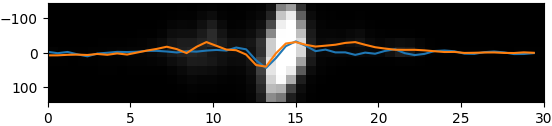
\includegraphics[width=\textwidth]{fig/doppler_1182}
					\end{subfigure}
					~ 
					\begin{subfigure}[t]{0.49\textwidth}
						\centering
						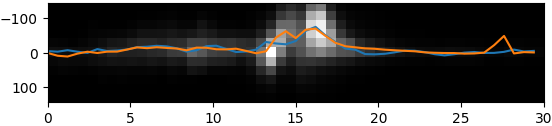
\includegraphics[width=\textwidth]{fig/doppler_1225}
					\end{subfigure}
					~ 
					\begin{subfigure}[t]{0.49\textwidth}
						\centering
						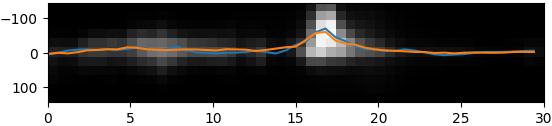
\includegraphics[width=\textwidth]{fig/doppler_1263}
					\end{subfigure}
					~ 
					\begin{subfigure}[t]{0.49\textwidth}
						\centering
						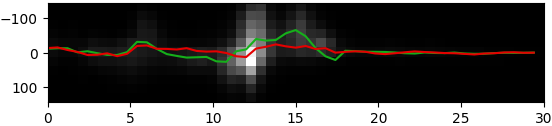
\includegraphics[width=\textwidth]{fig/doppler_1343}
					\end{subfigure}
					\caption{Examples of central-tendency inversions. Each image is an IRIS \SiIV spectra scaled into \MOSES resolution. The vertical axis is in km/s and the horizontal axis is in arcsec. The true line center is plotted in orange, and the reconstructed line center is plotted in blue.}
					\label{dopp_ex}
				\end{figure*}

			
				\begin{figure*}[h!]
					\centering
					\begin{subfigure}[t]{0.5\textwidth}
						\centering
						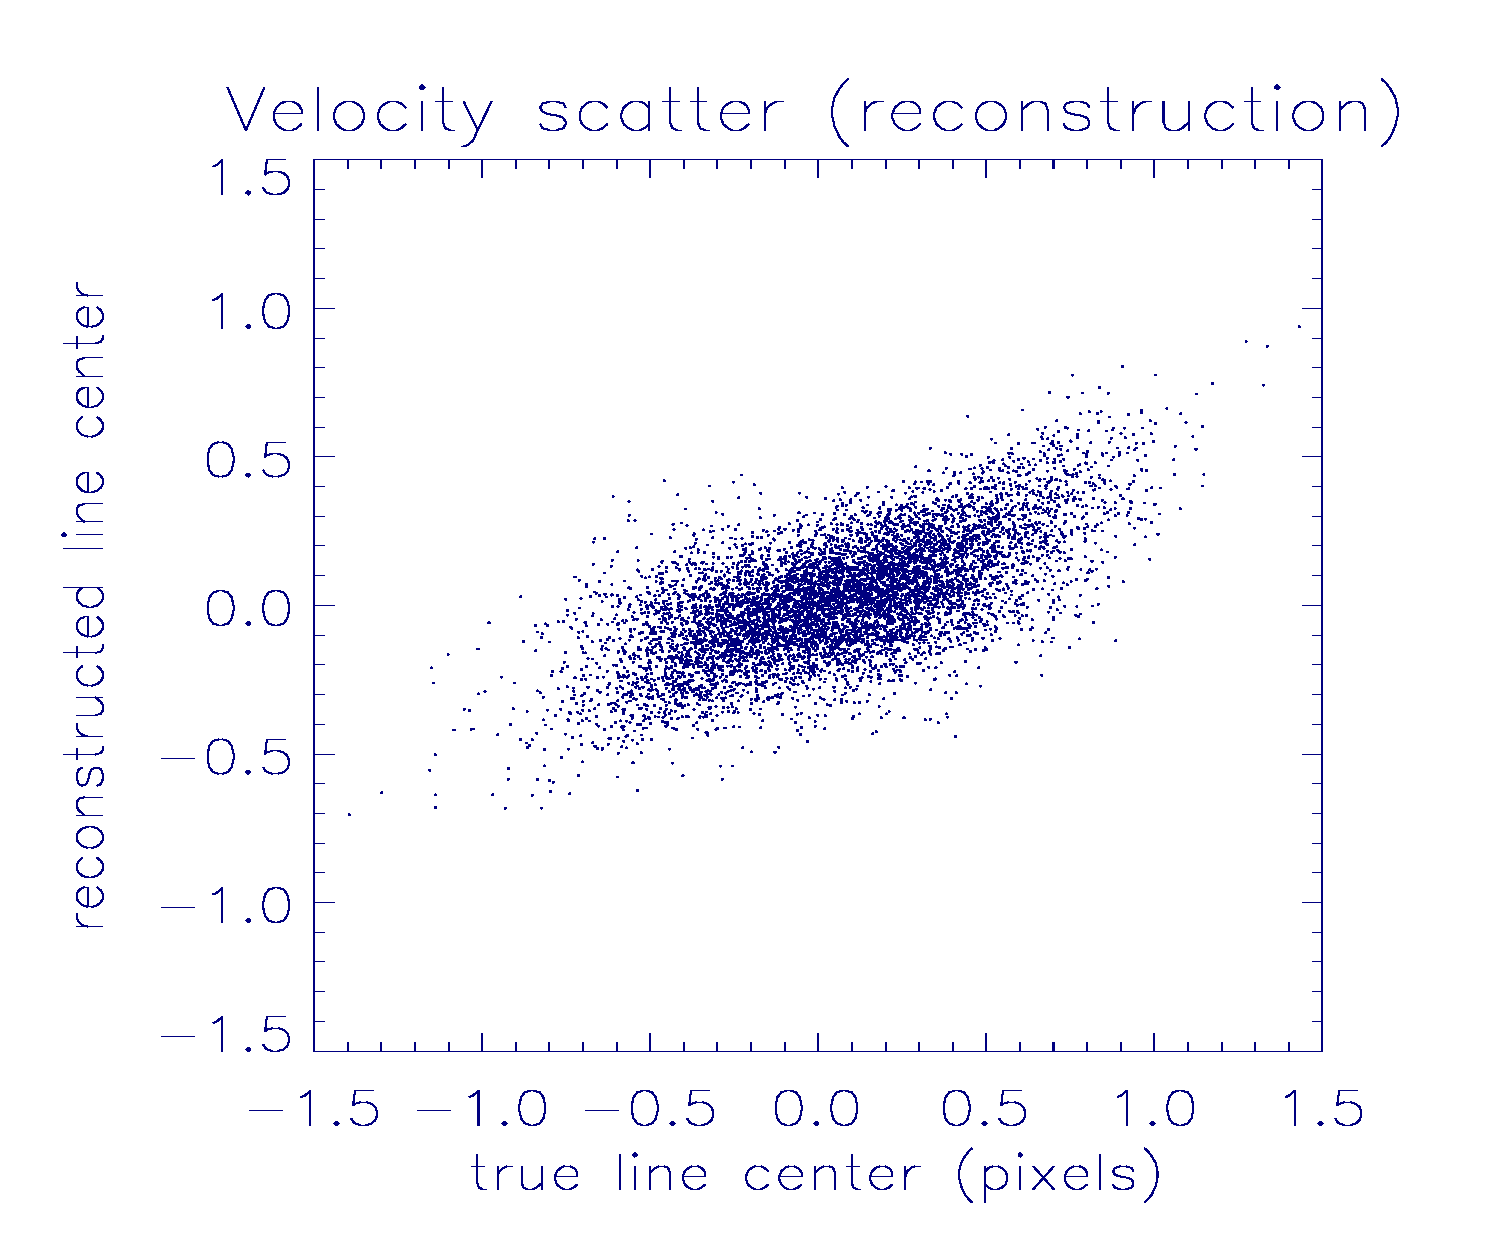
\includegraphics[width=\textwidth]{fig/smart_hist}
						\caption{SMART}
					\end{subfigure}%
					~ 
					\begin{subfigure}[t]{0.5\textwidth}
						\centering
						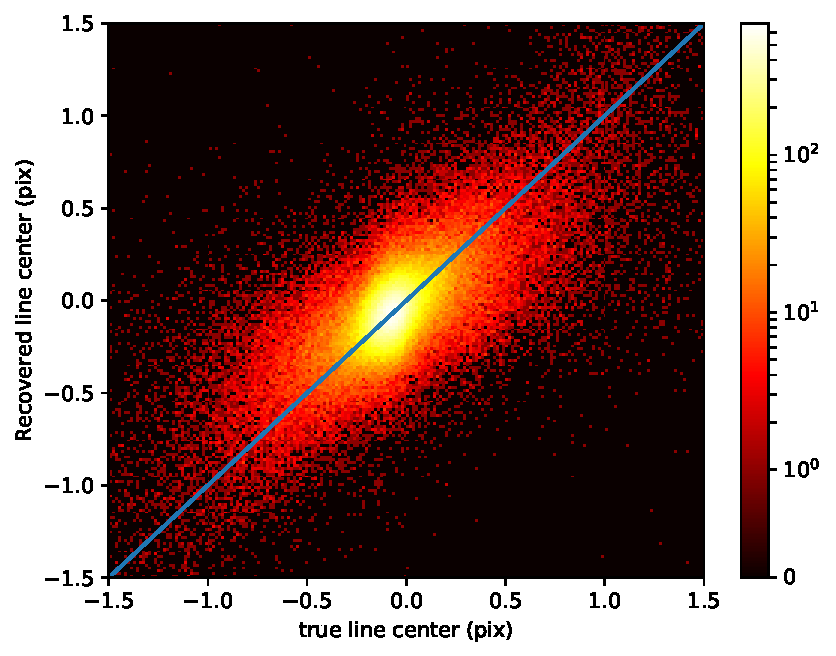
\includegraphics[width=\textwidth]{fig/linearity}
						\caption{CINN}
					\end{subfigure}
					\caption{Doppler velocity reconstruction using both the standard SMART algorithm (applied to SUMER O\,\textsc{iii} 703.87 \AA\ raster), and the CINN algorithm (applied to IRIS Si\,\textsc{iv} 1403 \AA.)}
					\label{dopp_hist}
				\end{figure*}
				

							
			\subsubsection{Despiking Training Data}	\label{sec_dspk}
			
				\begin{figure*}[h!]
					\centering
					\begin{subfigure}[t]{\textwidth}
						\centering
						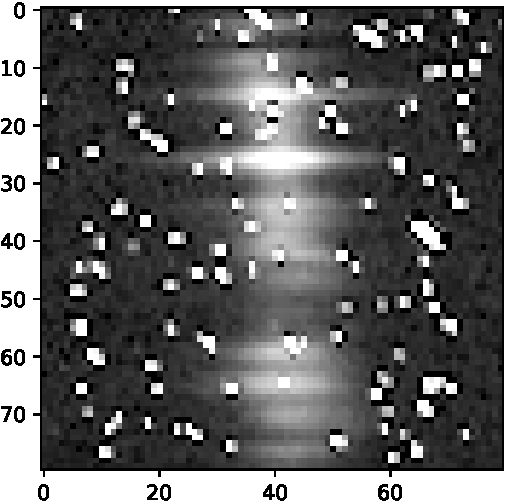
\includegraphics[width=\textwidth]{fig/orig}
					\end{subfigure}
					~ 
					\begin{subfigure}[t]{\textwidth}
						\centering
						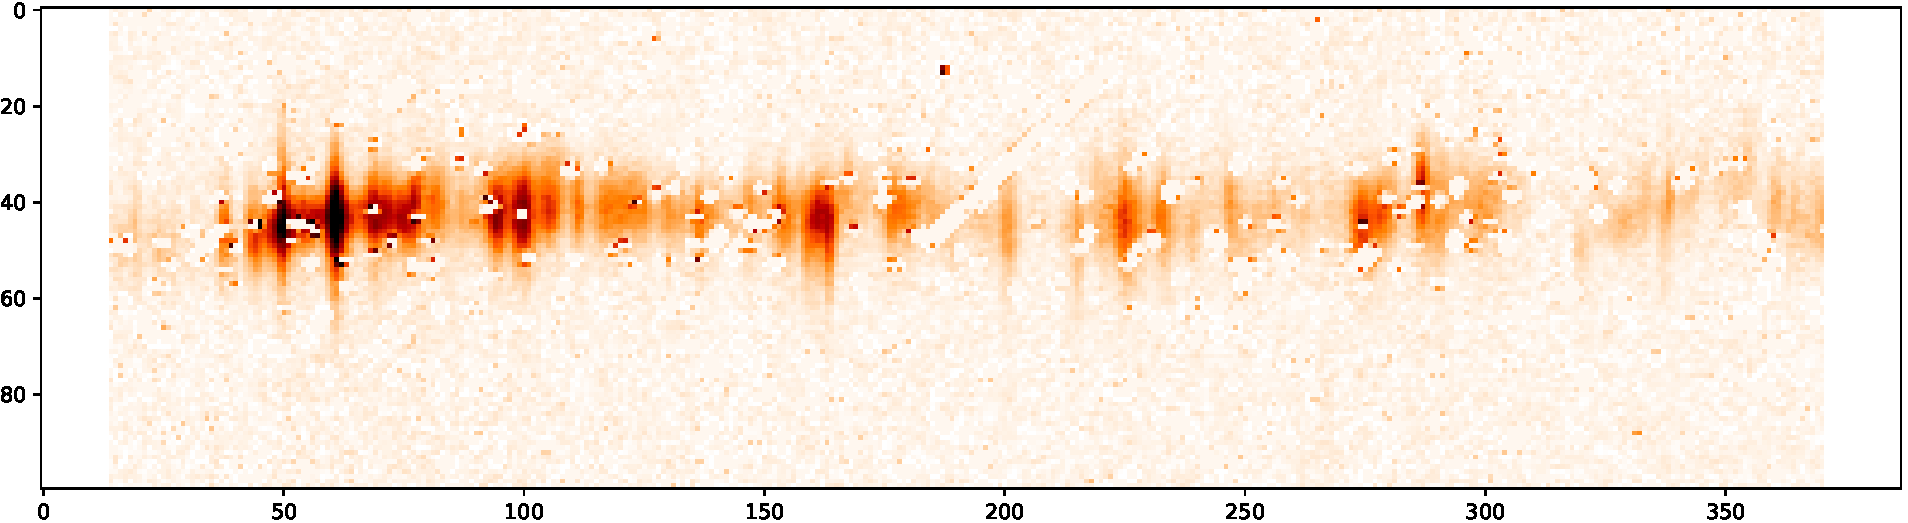
\includegraphics[width=\textwidth]{fig/dspk}
					\end{subfigure}
					\caption{An example of our despiking algorithm applied to an IRIS \SiIV spectra, the 47th frame of the observation gathered at 07:24:26 on 06-16-2015. The top image is the original data, and the bottom image is the original data with the identified spikes set to zero.}
				\end{figure*}
		
		\subsection{MOSES/ESIS Preparation}
		
		\subsection{FURST Design}
	
	\section{Proposal for Renewal}
	
		\subsection{Further CINN Development}
		
			\subsubsection{Training Data Pipeline}
		
			\subsubsection{Quantile Inversion Network}
			
			\subsection{Generative-Adversarial Networks}	\label{sec_gan}
		
		\subsection{Explosive Event Classification}
		
			
		
		\subsection{MOSES/ESIS Launch}
		
		\subsection{Publications}
	
	\section{Conclusion}
	
\end{document}